
\bta{2013}



\section{Use of English}

\noindent
\textbf{Directions:}\\
Read the following text. Choose the best word (s) for each
	numbered blank and mark A, B, C or D on \textbf{ANSWER SHEET 1}. (10 points)



\TiGanSpace


People are, on the whole, poor at considering background information
when making individual decisions. At first glance this might seem like a
strength that \cloze the ability to make judgments which are
unbiased by \cloze factors. But Dr. Uri Simonsohn speculated that
an inability to consider the big \cloze was leading
decision-makers to be biased by the daily samples of information they
were working with. \cloze , he theorised that a
judge \cloze of appearing too soft \cloze crime might be
more likely to send someone to prison \cloze he had already
sentenced five or six other defendants only to forced community service
on that day.

To \cloze this idea, he turned to the university-admissions
process. In theory, the \cloze of an applicant should not depend
on the few others \cloze randomly for interview during the same
day, but Dr. Simonsoho suspected the truth was \cloze.

He studied the results of 9, 323 MBA interviews \cloze by 31
admissions officers. The interviewers had \cloze applicants on a
scale of one to five. This scale \cloze numerous factors into
consideration. The scores were \cloze used in conjunction with
an applicant's score on the Graduate Management Admission Test, or GMAT,
a standardized exam which is \cloze out of 800 points, to make a
decision on whether to accept him or her.

Dr. Simonsohn found if the score of the previous candidate in a daily
series of interviewees was 0.75 points or more higher than that of the
one \cloze that, then the score for the next applicant
would \cloze by an average of 0.075 points. This might sound
small, but to \cloze the effects of such a decrease a candidate
would need 30 more GMAT points than would otherwise have
been \cloze.



\newpage

\begin{enumerate}
	%\renewcommand{\labelenumi}{\arabic{enumi}.}
	% A(\Alph) a(\alph) I(\Roman) i(\roman) 1(\arabic)
	%设定全局标号series=example	%引用全局变量resume=example
	%[topsep=-0.3em,parsep=-0.3em,itemsep=-0.3em,partopsep=-0.3em]
	%可使用leftmargin调整列表环境左边的空白长度 [leftmargin=0em]
	\item


\fourchoices
{grants}
{submits}
{transmits}
{delivers}




\item


\fourchoices
{minor}
{objective}
{crucial}
{external}




\item


\fourchoices
{issue}
{vision}
{picture}
{moment}




\item


\fourchoices
{For example}
{On average}
{In principle}
{Above all}





\item


\fourchoices
{fond}
{fearful}
{capable}
{thoughtless}




\item


\fourchoices
{in}
{on}
{to}
{for}






\item


\fourchoices
{if}
{until}
{though}
{unless}




\item


\fourchoices
{promote}
{emphasize}
{share}
{test}




\item


\fourchoices
{decision}
{quality}
{status}
{success}




\item


\fourchoices
{chosen}
{studied}
{found}
{identified}




\item

\fourchoices
{exceptional}
{defensible}
{replaceable}
{otherwise}


\item


\fourchoices
{inspired}
{expressed}
{conducted}
{secured}




\item


\fourchoices
{assigned}
{rated}
{matched}
{arranged}




\item


\fourchoices
{put}
{got}
{gave}
{took}





\item


\fourchoices
{instead}
{then}
{ever}
{rather}




\item


\fourchoices
{selected}
{passed}
{marked}
{introduced}




\item


\fourchoices
{before}
{after}
{above}
{below}







\item


\fourchoices
{jump}
{float}
{drop}
{fluctuate}



\item


\fourchoices
{achieve}
{undo}
{maintain}
{disregard}




\item


\fourchoices
{promising}
{possible}
{necessary}
{helpful}

\end{enumerate}


\vfil

\section{Reading Comprehension}


\noindent
\textbf{Part A}\\
\textbf{Directions:}\\
Read the following four texts. Answer the questions below each
	text by choosing A, B, C or
	D. Mark your answers on \textbf{ANSWER SHEET 1}. (40
	points)

\newpage
\subsection{Text 1}


In the 2006 film version of \emph{The Devil Wears Prada}, Miranda
Priestly, played by Meryl Streep, scolds her unattractive assistant for
imagining that high fashion doesn't affect her. Priestly explains how
the deep blue color of the assistant's sweater descended over the years
from fashion shows to department stores and to the bargain bin in which
the poor girl doubtless found her garment.

This top-down conception of the fashion business couldn't be more out of
date or at odds with the feverish world described
in \emph{Overdressed,} Elizabeth Cline's
three-year \uline{indictment} of ``fast fashion''. In the last
decade or so, advances in technology have allowed mass-market labels
such as Zara, H\&M, and Uniqlo to react to trends more quickly and
anticipate demand more precisely. Quicker turnarounds mean less wasted
inventory, more frequent releases, and more profit. These labels
encourage style-conscious consumers to see clothes as disposable---meant
to last only a wash or two, although they don't advertise that---and to
renew their wardrobe every few weeks. By offering on-trend items at
dirt-cheap prices, Cline argues, these brands have hijacked fashion
cycles, shaking an industry long accustomed to a seasonal pace.

The victims of this revolution, of course, are not limited to designers.
For H\&M to offer a \$5.95 knit miniskirt in all its 2, 300-plus stores
around the world, it must rely on low-wage overseas labor, order in
volumes that strain natural resources, and use massive amounts of
harmful chemicals.

\emph{Overdressed} is the fashion world's answer to consumer-activist
bestsellers like Michael Pollan's \emph{The Omnivore's Dilemma}.
``Mass-produced clothing, like fast food, fills a hunger and need, yet
is non-durable and wasteful,'' Cline argues. Americans, she finds, buy
roughly 20 billion garments a year---about 64 items per person---and no
matter how much they give away, this excess leads to waste.

Towards the end of \emph{Overdressed}, Cline introduced her ideal, a
Brooklyn woman named Sarah Kate Beaumont, who since 2008 has made all of
her own clothes---and beautifully. But as Cline is the first to note, it
took Beaumont decades to perfect her craft; her example can't be knocked
off.

Though several fast-fashion companies have made efforts to curb their
impact on labor and the environment---including H\&M, with its green
Conscious Collection line---Cline believes lasting change can only be
effected by the customer. She exhibits the idealism common to many
advocates of sustainability, be it in food or in energy. Vanity is a
constant; people will only start shopping more sustainably when they
can't afford not to.



\begin{enumerate}[resume]
	%\renewcommand{\labelenumi}{\arabic{enumi}.}
	% A(\Alph) a(\alph) I(\Roman) i(\roman) 1(\arabic)
	%设定全局标号series=example	%引用全局变量resume=example
	%[topsep=-0.3em,parsep=-0.3em,itemsep=-0.3em,partopsep=-0.3em]
	%可使用leftmargin调整列表环境左边的空白长度 [leftmargin=0em]
	\item
Priestly criticizes her assistant for her \lineread.


\fourchoices
{poor bargaining skill}
{insensitivity to fashion}
{obsession with high fashion}
{lack of imagination}


\item
According to Cline, mass-market labels urge consumers to \lineread.


\fourchoices
{combat unnecessary waste}
{shut out the feverish fashion world}
{resist the influence of advertisements}
{shop for their garments more frequently}





\item
The word ``indictment'' (Line 3, Para. 2) is closest in
meaning to \lineread.


\fourchoices
{accusation}
{enthusiasm}
{indifference}
{tolerance}


\item
Which of the following can be inferred from the last
paragraph?


\fourchoices
{Vanity has more often been found in idealists.}
{The fast-fashion industry ignores sustainability.}
{People are more interested in unaffordable garments.}
{Pricing is vital to environment-friendly purchasing.}



\item
What is the subject of the text?


\fourchoices
{Satire on an extravagant lifestyle.}
{Challenge to a high-fashion myth.}
{Criticism of the fast-fashion industry.}
{Exposure of a mass-market secret}

\end{enumerate}

\newpage
\subsection{Text 2}


An old saying has it that half of all advertising budgets are
wasted---the trouble is, no one knows which half. In the internet age,
at least in theory, this fraction can be much reduced. By watching what
people search for, click on and say online, companies can aim
``behavioral'' ads at those most likely to buy.

In the past couple of weeks a quarrel has illustrated the value to
advertisers of such fine-grained information: Should advertisers assume
that people are happy to be tracked and sent behavioral ads? Or should
they have explicit permission?

In December 2010 America's Federal Trade Commission (FTC) proposed
adding a ``do not track'' (DNT) option to internet browsers, so that
users could tell advertisers that they did not want to be followed.
Microsoft's Internet Explorer and Apple's Safari both offer DNT;
Google's Chrome is due to do so this year. In February the FTC and
Digital Advertising Alliance (DAA) agreed that \uline{the
	industry} would get cracking on responding to DNT requests.

On May 31st Microsoft set off the row. It said that InternetExplorer 10,
the version due to appear with Windows 8, would have DNT as a default.

Advertisers are horrified. Human nature being what it is, most people
stick with default settings. Few switch DNT on now, but if tracking is
off it will stay off. Bob Liodice, the chief executive of the
Association of National Advertisers, says consumers will be worse off if
the industry cannot collect information about their preferences. People
will not get fewer ads, he says, ``they'll get less meaningful, less
targeted ads.''

It is not yet clear how advertisers will respond. Getting a DNT signal
does not oblige anyone to stop tracking, although some companies have
promised to do so. Unable to tell whether someone really objects to
behavioral ads or whether they are sticking with Microsoft's default,
some may ignore a DNT signal and press on anyway.

Also unclear is why Microsoft has gone it alone. After all, it has an ad
business too, which it says will comply with DNT requests, though it is
still working out how. If it is trying to upset Google, which relies
almost wholly on advertising, it has chosen an indirect method: There is
no guarantee that DNT by default will become the norm. DNT does not seem
an obviously huge selling point for Windows 8---though the firm has
compared some of its other products favorably with Google's on that
count before. Brendon Lynch, Microsoft's chief privacy officer, blogged:
``we believe consumers should have more control.'' Could it really be
that simple?



\begin{enumerate}[resume]
	%\renewcommand{\labelenumi}{\arabic{enumi}.}
	% A(\Alph) a(\alph) I(\Roman) i(\roman) 1(\arabic)
	%设定全局标号series=example	%引用全局变量resume=example
	%[topsep=-0.3em,parsep=-0.3em,itemsep=-0.3em,partopsep=-0.3em]
	%可使用leftmargin调整列表环境左边的空白长度 [leftmargin=0em]
	\item
 It is suggested in paragraph 1 that ``behavioral'' ads help
advertisers to \lineread.


\fourchoices
{ease competition among themselves}
{lower their operational costs}
{avoid complaints from consumers}
{provide better online services}


\item
``The industry'' (Line 5, Para. 3) refers to \lineread.


\fourchoices
{online advertisers}
{e-commerce conductors}
{digital information analysts}
{internet browser developers}



\item
Bob Liodice holds that setting DNT as a default \lineread.


\fourchoices
{may cut the number of junk ads}
{fails to affect the ad industry}
{will not benefit consumers}
{goes against human nature}


\item
 Which of the following is true according to Paragraph 6?


\fourchoices
{DNT may not serve its intended purpose}
{Advertisers are willing to implement DNT}
{DNT is losing its popularity among consumers}
{Advertisers are obliged to offer behavioral ads}





\item
The author's attitude towards what Brendon Lynch said in his
blog is one of \lineread.


\fourchoices
{indulgence}
{understanding}
{appreciation}
{skepticism}


\end{enumerate}


\newpage
\subsection{Text 3}


Up until a few decades ago, our visions of the future were
largely---though by no means uniformly---glowingly positive. Science and
technology would cure all the ills of humanity, leading to lives of
fulfillment and opportunity for all.

Now utopia has grown unfashionable, as we have gained a deeper
appreciation of the range of threats facing us, from asteroid strike to
epidemic flu to climate change. You might even be tempted to assume that
humanity has little future to look forward to.

But such gloominess is misplaced. The fossil record shows that many
species have endured for millions of years---so why shouldn't we? Take a
broader look at our species' place in the universe, and it becomes clear
that we have an excellent chance of surviving for tens, if not hundreds,
of thousands of years. Look up \emph{Homo sapiens} in the ``Red List''
of threatened species of the international Union for the Concentration
of Nature (IUCN), and you will read: ``Listed as Least Concern as the
species is very widely distributed, adaptable, currently increasing, and
there are no major threats resulting in an overall population decline.''

So what does our deep future hold? A growing number of researchers and
organizations are now thinking seriously about that question. For
example, the Long Now Foundation has as its flagship project a
mechanical clock that is designed to still be marking time thousands of
years hence.

Perhaps willfully, it may be easier to think about such lengthy
timescales than about the more immediate future. The potential evolution
of today's technology, and its social consequences, is dazzlingly
complicated, and it's perhaps best left to science fiction writers and
futurologists to explore the many possibilities we can envisage. That's
one reason why we have
launched \emph{Arc}, a new publication
dedicated to the near future.

But take a longer view and there is a surprising amount that we can say
with considerable assurance. As so often, the past holds the key to the
future: we have now identified enough of the long-term patterns shaping
the history of the planet, and our species, to make evidence-based
forecasts about the situations in which our descendants will find
themselves.

This long perspective makes the pessimistic view of our prospects seem
more likely to be a passing fad. To be sure, the future is not all rosy.
But we are now knowledgeable enough to reduce many of the risks that
threatened the existence of earlier humans, and to improve the lot of
those to come.

\begin{enumerate}[resume]
	%\renewcommand{\labelenumi}{\arabic{enumi}.}
	% A(\Alph) a(\alph) I(\Roman) i(\roman) 1(\arabic)
	%设定全局标号series=example	%引用全局变量resume=example
	%[topsep=-0.3em,parsep=-0.3em,itemsep=-0.3em,partopsep=-0.3em]
	%可使用leftmargin调整列表环境左边的空白长度 [leftmargin=0em]
	\item
Our vision of the future used to be inspired by \lineread.


\fourchoices
{our desire for lives of fulfillment}
{our faith in science and technology}
{our awareness of potential risks}
{our belief in equal opportunity}


\item
The IUCN's ``Red List'' suggests that human beings are \lineread.


\fourchoices
{a sustained species}
{a threat to the environment}
{the world's dominant power}
{a misplaced race}



\item
Which of the following is true according to Paragraph 5?


\fourchoices
{\emph{Arc} helps limit the scope of futurological studies.}
{Technology offers solutions to social problems.}
{The interest in science fiction is on the rise.}
{Our immediate future is hard to conceive.}



\item
To ensure the future of mankind, it is crucial to \lineread.


\fourchoices
{explore our planet's abundant resources}
{adopt an optimistic view of the world}
{draw on our experience from the past}
{curb our ambition to reshape history}


\item
Which of the following would be the best title for the
text?


\fourchoices
{Uncertainty about Our Future}
{Evolution of the Human Species}
{The Ever-bright Prospects of Mankind.}
{Science, Technology and Humanity.}

\end{enumerate}



\newpage
\subsection{Text 4}


On a five to three vote, the Supreme Court knocked out much of Arizona's
immigration law Monday---a modest policy victory for the Obama
Administration. But on the more important matter of the Constitution,
the decision was an 8-0 defeat for the Administration's effort to upset
the balance of power between the federal government and the states.

In Arizona v. United States, the majority overturned three of the
four contested provisions of Arizona's controversial plan to have state
and local police enforce federal immigration law. The Constitutional
principles that Washington alone has the power to ``establish a uniform
Rule of Naturalization'' and that federal laws precede state laws are
noncontroversial. Arizona had attempted to fashion state policies that
ran parallel to the existing federal ones.

Justice Anthony Kennedy, joined by Chief Justice John Roberts and the
Court's liberals, ruled that the state flew too close to the federal
sun. On the overturned provisions the majority held that Congress had
deliberately ``occupied the field'' and Arizona has thus intruded on the
federal's privileged powers.

However, the Justices said that Arizona police would be allowed to
verify the legal status of people who come in contact with law
enforcement. That's because Congress has always envisioned joint
federal-state immigration enforcement and explicitly encourages state
officers to share information and cooperate with federal colleagues.

Two of the three objecting Justices---Samuel Alito and Clarence
Thomas---agreed with this Constitutional logic but disagreed about which
Arizona rules conflicted with the federal statute. The only major
objection came from Justice Antonin Scalia, who offered an even more
robust defense of state privileges going back to the Alien and Sedition
Acts.

The 8-0 objection to President Obama turns on what Justice Samuel Alito
describes in his objection as ``a shocking assertion of federal
executive power''. The White House argued that Arizona's laws conflicted
with its enforcement priorities, even if state laws complied with
federal statutes to the letter. In effect, the White House claimed that
it could invalidate any otherwise legitimate state law that it disagrees
with.

Some powers do belong exclusively to the federal government, and control
of citizenship and the borders is among them. But if Congress wanted to
prevent states from using their own resources to check immigration
status, it could. It never did so. The Administration was in essence
asserting that because it didn't want to carry out Congress's
immigration wishes, no state should be allowed to do so either. Every
Justice rightly rejected this remarkable claim.


\begin{enumerate}[resume]
	%\renewcommand{\labelenumi}{\arabic{enumi}.}
	% A(\Alph) a(\alph) I(\Roman) i(\roman) 1(\arabic)
	%设定全局标号series=example	%引用全局变量resume=example
	%[topsep=-0.3em,parsep=-0.3em,itemsep=-0.3em,partopsep=-0.3em]
	%可使用leftmargin调整列表环境左边的空白长度 [leftmargin=0em]
	\item
Three provisions of Arizona's plan were overturned because
they \lineread.


\fourchoices
{deprived the federal police of Constitutional powers}
{disturbed the power balance between different states}
{overstepped the authority of federal immigration law}
{contradicted both the federal and state policies}



\item
On which of the following did the Justices agree, according
to Paragraph 4?


\fourchoices
{Federal officers' duty to withhold immigrants' information.}
{States' independence from federal immigration law.}
{States' legitimate role in immigration enforcement.}
{Congress's intervention in immigration enforcement.}



\item
It can be inferred from Paragraph 5 that the Alien and
Sedition Acts \lineread.


\fourchoices
{violated the Constitution}
{undermined the states' interests}
{supported the federal statute}
{stood in favor of the states}


\item
The White House claims that its power of enforcement \lineread.


\fourchoices
{outweighs that held by the states}
{is dependent on the states' support}
{is established by federal statutes}
{rarely goes against state laws}


\item
What can be learned from the last paragraph?


\fourchoices
{Immigration issues are usually decided by Congress.}
{The Administration is dominant over immigration issues.}
{Justices wanted to strengthen its coordination with Congress.}
{Justices intended to check the power of the Administration.}



	
\end{enumerate}


\newpage

\noindent
\textbf{Part B}\\
\textbf{Directions:}\\
In the following article, some sentences have been removed. For
	Questions 41-45, choose the most suitable one from the list A-G to fit
	into each of the numbered blank. There are two extra choices, which do
	not fit in any of the gaps. Mark your answers on \textbf{ANSWER SHEET 1}. (10 points)


\TiGanSpace


The social sciences are flourishing. As of 2005, there were almost half
a million professional social scientists from all fields in the world,
working both inside and outside academia. According to the \emph{World
	Social Science Report 2010}, the number of social-science students
worldwide has swollen by about 11\% every year since 2000.

Yet this enormous resource is not contributing enough to today's global
challenges, including climate change, security, sustainable development
and health.  
\linefill.
Humanity has
the necessary agro-technological tools to eradicate hunger, from
genetically engineered crops to artificial fertilizers. Here, too, the
problems are social: the organization and distribution of food, wealth
and prosperity.




\linefill. This is a shame---the
community should be grasping the opportunity to raise its influence in
the real world. To paraphrase the great social scientist Joseph
Schumpeter: there is no radical innovation without creative destruction.

Today, the social sciences are largely focused on disciplinary problems
and internal scholarly debates, rather than on topics with external
impact. Analyses reveal that the number of papers including the keywords
``environmental change'' or ``climate change'' have increased rapidly
since 2004. \linefill.

When social scientists do tackle practical issues, their scope is often
local: Belgium is interested mainly in the effects of poverty on
Belgium, for example. And whether the community's work contributes much
to an overall accumulation of knowledge is doubtful.

The problem is not necessarily the amount of available funding. \linefill. This is an adequate amount so
long as it is aimed in the right direction. Social scientists who
complain about a lack of funding should not expect more in today's
economic climate.

The trick is to direct these funds better. The European Union Framework
funding programs have long had a category specifically targeted at
social scientists. This year, it was proposed that the system be
changed: Horizon 2020, a new program to be enacted in 2014, would not
have such a category. This has resulted in protests from social
scientists. But the intention is not to neglect social science; rather,
the complete opposite. \linefill.
That should create more collaborative endeavors and help to develop
projects aimed directly at solving global problems.

\begin{listmatch}
	%\renewcommand{\labelenumi}{\arabic{enumi}.}
	% A(\Alph) a(\alph) I(\Roman) i(\roman) 1(\arabic)
	%设定全局标号series=example	%引用全局变量resume=example
	%[topsep=-0.3em,parsep=-0.3em,itemsep=-0.3em,partopsep=-0.3em]
	%可使用leftmargin调整列表环境左边的空白长度 [leftmargin=0em]
	\item
 It could be that we are evolving two communities of social
scientists: one that is discipline-oriented and publishing in highly
specialized journals, and one that is problem-oriented and publishing
elsewhere, such as policy briefs.


\item 
 However, the numbers are still small: in 2010, about 1, 600 of
the 100, 000 social-sciences papers published globally included one of
these keywords.

\item 
The idea is to force social scientists to integrate their work
with other categories, including health and demographic change; food
security; marine research and the bio-economy, clean, efficient energy;
and inclusive, innovative and secure societies.





\item 
The solution is to change the mindset of the academic community,
and what it considers to be its main goal. Global challenges and social
innovation ought to receive much more attention from scientists,
especially the young ones.

\item 
These issues all have root causes in human behavior: all require
behavioral change and social innovations, as well as technological
development. Stemming climate change, for example, is as much about
changing consumption patterns and promoting tax acceptance as it is
about developing clean energy.


\item 
Despite these factors, many social scientists seem reluctant to
tackle such problems. And in Europe, some are up in arms over a proposal
to drop a specific funding category for social-science research and to
integrate it within cross-cutting topics of sustainable development.




\item 
During the late 1990s , national spending on social sciences and
the humanities as a percentage of all research and development
funds---including government, higher education, non-profit and
corporate---varied from around 4\% to 25\%; in most European nations, it
is about 15\%.








\end{listmatch}



\newpage
\noindent
\textbf{Part C}\\
\textbf{Directions:}\\
Read the following text carefully and then translate the
	underlined segments into Chinese. Your translation should be written
	clearly on \textbf{ANSWER SHEET 2}. (10 points)



\TiGanSpace



It is speculated that gardens arise from a basic human need in the
individuals who made them: the need for creative expression. There is no
doubt that gardens evidence an irrepressible urge to create, express,
fashion, and beautify and that self-expression is a basic human urge;
\transnum \uline{yet when one looks at the photographs of the garden
	created by the homeless, it strikes one that , for all their diversity of
	styles, these gardens speak of various other fundamental urges, beyond
	that of decoration and creative expression.}

One of these urges has to do with creating a state of peace in the midst
of turbulence, a ``still point of the turning world,'' to borrow a
phrase from T. S. Eliot. \transnum \uline{A sacred place of peace,
	however crude it may be, is a distinctly human need, as opposed to
	shelter, which is a distinctly animal need.} This distinction is so much
so that where the latter is lacking, as it is for these unlikely
gardens, the former becomes all the more urgent. Composure is a state of
mind made possible by the structuring of one's relation to one's
environment. \transnum \uline{The gardens of the homeless, which are in
	effect homeless gardens, introduce form into an
	urban environment where it either didn't exist or was not discernible as
	such.} In so doing they give composure to a segment of the inarticulate
environment in which they take their stand.

Another urge or need that these gardens appear to respond to, or to
arise from, is so intrinsic that we are barely ever conscious of its
abiding claims on us. When we are deprived of green, of plants, of
trees, \transnum \uline{ most of us give in to a demoralization of spirit
	which we usually blame on some psychological conditions, until one day
	we find ourselves in a garden and feel the oppression vanish as if by
	magic.} In most of the homeless gardens of New York City the actual
cultivation of plants is unfeasible, yet even so the compositions often
seem to represent attempts to call forth the spirit of plant and animal
life, if only symbolically, through a clumplike arrangement of
materials, an introduction of colors, small pools of water, and a
frequent presence of petals or leaves as well as of stuffed animals. On
display here are various fantasy elements whose reference, at some basic
level, seems to be the natural world. \transnum \uline{It is this
	implicit or explicit reference to nature that fully justifies the use of
	the word garden, though in a ``liberated''
	sense, to describe these synthetic constructions.} In them we can see
biophilia---a yearning for contact with nonhuman life---assuming uncanny
representational forms.

\newpage

\section{Writing}


\noindent
\textbf{Part A}\\
\textbf{51. Directions:}

Write an e-mail of about 100 words to a foreign teacher in your college,
inviting him/her to be a judge for the upcoming English speech contest.

You should include the details you think necessary.

You should write neatly on the ANSWER SHEET 2.

\textbf{Do not} sign your own name at the end of the e-mail. Use ``Li Ming''
instead.

\textbf{Do not} write the address. (10 points)



\vspace{3em}

\noindent
\textbf{Part B}\\
\textbf{52. Directions:}

Write an essay of 160-200 words based on the following drawing. In your
essay you should
\begin{listwrite}
	%\renewcommand{\labelenumi}{\arabic{enumi}.}
	% A(\Alph) a(\alph) I(\Roman) i(\roman) 1(\arabic)
	%设定全局标号series=example	%引用全局变量resume=example
	%[topsep=-0.3em,parsep=-0.3em,itemsep=-0.3em,partopsep=-0.3em]
	%可使用leftmargin调整列表环境左边的空白长度 [leftmargin=0em]
	\item
	describe the drawing briefly

\item 
 explain its intended meaning, and

\item 
 give your comments.
\end{listwrite}

You should write neatly on the ANSWER SHEET 2. (20 points)


\begin{figure}[h!]
	\centering
	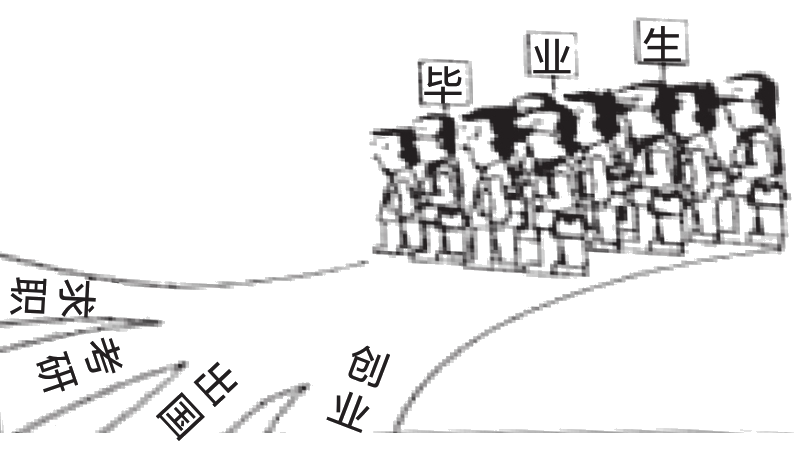
\includegraphics[width=0.56\linewidth]{picture/2013.png}
	\caption*{选择}
\end{figure}

\checkpagenumber